% \chapter{Virtual Knots}
% \section{Introduction}
% While the diagram graph defined in the previous chapter is a nice
% computational tool for manipulating knots, from a more theoretical
% standpoint, it leaves quite a bit to be desired.

% Ultimately, our purpose with the signed Gauss code was to try and
% identify a cleaner algebraic way of understanding knot theory in terms
% of purely combinatorial structure. Unfortunately, the planarity
% restrictions we had to place on Reidemeister II make it hard to see
% this panning out. What are we to do? We have a few options:
% \begin{enumerate}[label=\arabic*)]
%   \item Abandon the signed Gauss code approach and search for
%     something more fruitful,
%   \item Double down on it and work at building up a rich theory around
%     the diagram graph, or
%   \item Extend our interpretation of ``knot'' to a new context where
%     we don't \emph{have} to worry about planarity concerns at all.
% \end{enumerate}
% We'll choose option (3). Here, this will lead us to the field of
% \emph{virtual knot theory} (\cite{Kauffman1998Nov}). The idea is to
% make signed Gauss codes our fundamental object of study, without
% including any concerns about planarity conditions. We'll give two
% small pieces of motivation before getting into the thick of it. One
% draws an analogy with defining the complex numbers, the other with
% drawing planar graphs on surfaces
% other than $\RR^2$.\\

% \noindent \textbf{Question 1} (Motivation)\textbf{.} Is it possible to
% find an $x$ such that $x^2 = -1$?
% \begin{leftbar}
%   \begin{sproof}[Answer 1.]
%     No. For any $x \in \RR$ we have $x^2 \geq 0$. Hence such an $x$
%     doesn't exist.
%   \end{sproof}
% \end{leftbar}
% But of course, we could use complex numbers instead to make things
% work out.
% \begin{leftbar}
%   \begin{sproof}[Answer 2.]
%     Define a new symbol $i$ such that $i^2 = -1$. Then this gives the
%     desired $x$.\footnote{Or, for a more algebraic point of view,
%       instead of thinking ``$i^2 = -1$'' we can view $\CC$ as working
%       in $\RR[i]/\ip{i^2 + 1}$. Same end result, but the explicit
%       focus on modding out by an ideal might carry a different flavor
%       for some people.}
%   \end{sproof}
% \end{leftbar}
% While we often take the complex numbers for granted, it's important to
% recognize that at first glance defining $i^2 = -1$ might seem like
% nonsense --- or at the very least, a cop-out. But after years of
% careful study, we now know that $\CC$ can be very intuitive, and in
% many ways is actually nicer than $\RR$. For instance, every polynomial
% in $\CC$ of degree $n$ has $n$ roots in $\CC$. The same property is
% not enjoyed by the real numbers.

% This is analogous to the relationship between \emph{classical knots}
% (the things we have been referring to as ``knots'' up to this point)
% and \emph{virtual knots}. With virtual knots, every Gauss code has a
% corresponding knot. With \emph{classical} knots, we can sometimes get
% Gauss codes that are comparable to $x^2 = -1$ --- unless we extend our
% scope, it seems like there's no way to make sense of the statement.
% This extension will come from loosening the planarity constraints on
% the signed Gauss code. How are we to interpret the result? To start,
% consider the following question.\\

% \noindent \textbf{Question 2}
% (Motivation)\textbf{.}\hypertarget{question-2}{} Is it possible to
% draw the $K_{3,3}$ graph without any edge crossings?
% \begin{figure}[H]
%   \centering
%   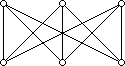
\includegraphics[scale=2.5]{\figdir/k-3-3.pdf}
%   \caption{The $K_{3,3}$ graph.}
%   \label{fig:k-3-3}
% \end{figure}
% We'll examine two answers to this question.
% \begin{leftbar}
%   \begin{sproof}[Answer 1]
%     No. One can show that in a planar graph, if there are no cycles of
%     length 3, then $\abs{E} \leq 2\abs{V} - 4$. For $K_{3,3}$, one can
%     verify that $\abs{E} = 9$ and $\abs{V = 6}$. But $9 \not\leq
%     2\cdot 6 - 4 = 8$, so $K_{3,3}$ is non-planar. Hence it cannot be
%     drawn without edge crossings.
%   \end{sproof}
% \end{leftbar}
% Nice! Rigorous, sensible, and to-the-point. Here's another answer.
% \begin{leftbar}
%   \begin{sproof}[Answer 2]
%     Yeah just draw it on a donut.
%   \end{sproof}
% \end{leftbar}
% \begin{figure}[H]
%   \centering
%   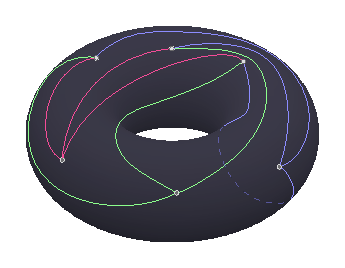
\includegraphics[draft]{\figdir/k-3-3-on-torus.pdf}
% \end{figure}

% \section{Definitions}
% We define (oriented) \emph{virtual knots} in terms of signed Gauss
% codes.
% \begin{definition}[Virtual Knot]
%   A \emph{virtual knot} is a string $\sigma$ of $2n$ characters such
%   that for each $k = 1, \ldots, n$, for some choice of $\epsilon_k \in
%   \set{+, -}$, the symbols $k^{\epsilon_k}_u$, $k^{\epsilon_k}_o$
%   each appear in $\sigma$ exactly once.
% \end{definition}
% Compare with \cref{def:signed-gauss-code}. Here, instead of defining
% Gauss codes in terms of knots, we've defined knots in terms of Gauss
% codes. Returning to our analogy with $\CC$ and $\RR$, this would be
% like defining $\CC$ as ``the set of all roots of single-variable
% polynomials with real coefficients.''\footnote{To see this, note that
%   for any $z \in \CC$, $(x - z) \cdot (x - \ol{z})$ has real
%   coefficients.}

% We define equivalence for virtual knots as follows:
% \begin{definition}[Equivalence of Virtual Knots]
%   We say two virtual knots $K_1$, $K_2$ are \emph{equivalent} if $K_1$
%   can be transformed into $K_2$ by a finite sequence of Gauss code
%   Reidemeister moves (this time without the planarity constraints on
%   Reidemeister II).
% \end{definition}
% How do we interpret virtual knots and their equivalence geometrically?
% Treating this question in full would take us beyond the scope of our
% purposes today, but we will give a high-level overview.\footnote{For
%   more, the reader is encouraged to investigate \cite{Carter2002May}}
% Our first order of business is to define virtual knot diagrams.
% \begin{definition}[Virtual knot diagram]
%   A \emph{virtual knot diagram} is defined identically to the
%   classical case, only now we include special \emph{virtual}
%   crossings that we insert whenever we're forced to violate planarity
%   to connect strands together. Virtual crossings are denoted by
%   circles, as in \cref{fig:virtual-crossing}.
% \end{definition}
% \begin{figure}[H]
%   \centering
%   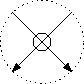
\includegraphics[scale=1.5]{\figdir/virtual-crossing.pdf}
%   \caption{A virtual crossing}
%   \label{fig:virtual-crossing}
% \end{figure}
% \begin{note}
%   Virtual crossings do not appear in the signed Gauss code. This is
%   because there's a sense in which they're not really ``there'' ---
%   rather, they're an artifact of our projection into $\RR^2$. We'll
%   expand on this below.
% \end{note}
% \begin{example}
%   Consider the virtual knot given by $1^+_o 2^+_o 1^+_u 2^+_u$. If we
%   were to try and interpret this as a classical knot, we'd run into
%   some problems:
%   \begin{figure}[H]
%     \centering
%     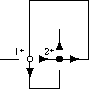
\includegraphics[scale=1.5]{\figdir/virtual-knot-example-classical.pdf}
%     \caption{Now what?}
%   \end{figure}
%   Note, there's no way to connect the strand to crossing $2$ in the
%   desired manner without introducing a \emph{new} crossing along the
%   $(2^+_o, 1^+_o)$ semiarc. Hence, we employ a virtual crossing, which
%   allows us to complete the diagram without problems.
%   \begin{figure}[H]
%     \centering
%     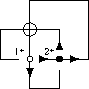
\includegraphics[scale=1.5]{\figdir/virtual-knot-example.pdf}
%     \caption{Virtual diagram}
%     \label{fig:virtual-trefoil-grid-diagram}
%     \qedhere
%   \end{figure}
% \end{example}
% How do we interpret the resulting ``knot'' as an embedding? A hint
% comes from \hyperlink{question-2}{\textbf{Motivating Question 2}}. As
% we saw there, it's still possible to draw $K_{3,3}$ without having
% edges cross each other if we work on a torus. Recalling the connection
% between signed Gauss codes and planar graphs that we established
% through the \hyperlink{def:diagram-graph}{diagram graph}, it seems
% reasonable to think of virtual knots as knots that we draw on
% thickened surfaces.\footnote{We need $[-\varepsilon, \varepsilon]$ of
%   wiggle room to let the strands pass over/under each other.} In this
% context, we see that virtual crossings don't really represent
% \emph{real} crossings of the strands in our knot. Rather, they're
% artifacts of our $2$D representations.
% \begin{figure}[H]
%   \centering
%   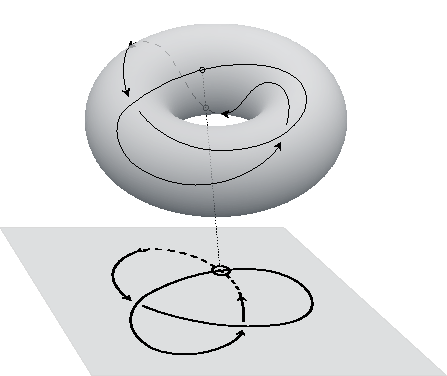
\includegraphics[scale=1.2]{\figdir/virtual-knot-on-torus.pdf}
%   \caption{An example of how we might obtain something like
%     \cref{fig:virtual-trefoil-grid-diagram}.}
%   \label{fig:virtual-projection}
% \end{figure}
% Some care has to be taken in reworking our interpretation of what it
% means for knots to be ``equivalent'' in this new context --- e.g., it
% seems we might be able to get two inequivalent unknots by drawing
% closed loops longitudinally / latitudinally on the surface. We will
% not worry too much about this today; we're only interested in the
% combinatorial aspects. For more, the reader is encouraged to look at
% \cite{Carter2002May}.

% By carefully studying \cref{fig:virtual-projection}, the reader might
% realize that performing Reidemeister moves on the surface of the torus
% can actually introduce extra virtual crossings into our $2$D
% projection.\footnote{This can also be derived entirely from looking at
%   the signed Gauss code Reidemeister moves without planarity
%   constraints.} This suggests that the purely diagrammatic
% Reidemeister moves are insufficient for manipulating virtual
% diagrams.\footnote{Of course, by definition the signed Gauss code
%   Reidemeister moves still suffice for virtual equivalence.} Indeed
% this is the case. The expanded moveset is given by adding the
% following four operations:
% \begin{figure}[H]
%   \centering
%   \begin{subfigure}[t]{0.5\textwidth}
%     \centering
%     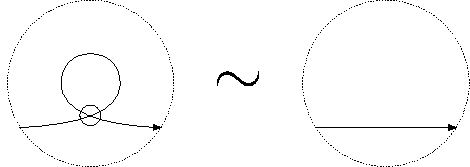
\includegraphics[scale=.575]{\figdir/virtual-r1.pdf}
%     \caption{Virtual Reid.\ I}
%     \label{fig:virtual-r1}
%   \end{subfigure}%
%   ~
%   \begin{subfigure}[t]{0.5\textwidth}
%     \centering
%     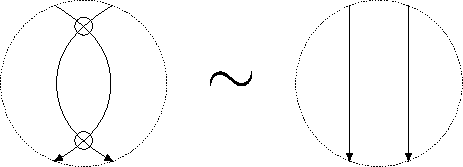
\includegraphics[scale=.575]{\figdir/virtual-r2.pdf}
%     \caption{Virtual Reid.\ II}
%   \end{subfigure}\\[1.5em]
%   \begin{subfigure}[t]{0.5\textwidth}
%     \centering
%     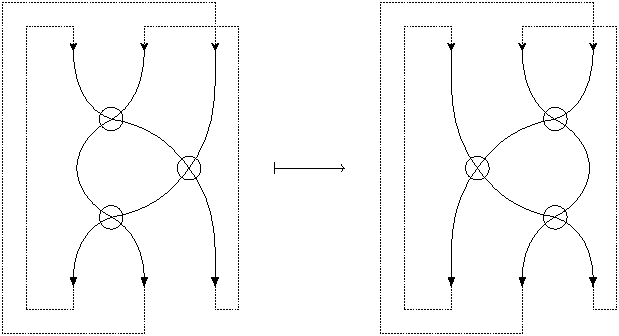
\includegraphics[scale=.5]{\figdir/virtual-r3.pdf}
%     \caption{Virtual Reid.\ III}
%     \label{fig:virtual-r1}
%   \end{subfigure}%
%   ~
%   \begin{subfigure}[t]{0.5\textwidth}
%     \centering
%     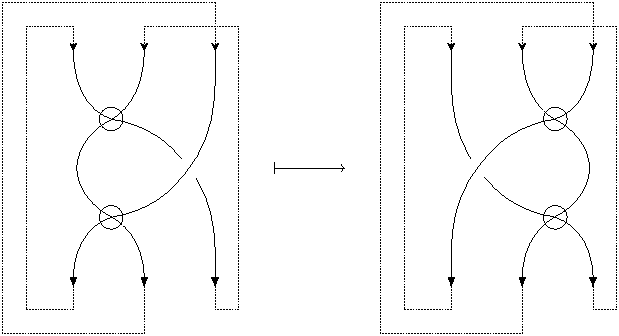
\includegraphics[scale=.5]{\figdir/virtual-r4.pdf}
%     \caption{Mixed Reid.\ III}
%   \end{subfigure}
%   \caption{The virtual moves}
% \end{figure}
% Together with the 3 standard diagrammatic Reidemeister moves, these
% are sufficient to fully encode equivalence of virtual knots.

% {\color{blue} Does anything else need to be done in this section?}

% % \subsection{Connected Sum}
% \begin{definition}[Connected Sum]
%   Let $K_0, K_1$ be knots, with associated diagrams $D_0, D_1$. Then
%   we define the \emph{connected sum} of $K_0$, $K_1$ by slicing $D_0,
%   D_1$ along an arc, and gluing the ends together.
% \end{definition}
% \begin{figure}[H]
%   \centering
%   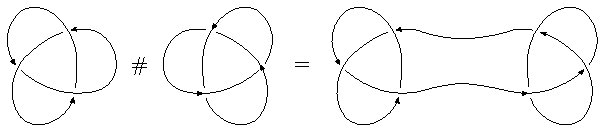
\includegraphics{figures/background/conn_sum.pdf}
%   \caption{Example of the connected sum}
% \end{figure}
% \noindent We can understand this operation as inserting one signed Gauss code
% into the middle of another.

% {\color{blue} introduce the connected sum}







% % We mentioned earlier that the diagram graph has some nice
% % computational properties.

% % \subsubsection{Unknotting moves and \#}
% % As we discussed in the introduction section, we want to create
% % algebraic structures to better understand how to build knots. The two
% % most popular such operations are \emph{unknotting moves}, which let us
% % reduce any knot diagram to the \emph{unknot}; and the \emph{connected
% %   sum} (denoted $\#$), which sort of acts like a ``multiplication''
% % operation on knots.

% % \begin{definition}[Unknotting move]
% %   An \emph{unknotting move} $u$ is a local modification of a diagram
% %   such that $u$ together with the Reidemeister moves is sufficient to
% %   reduce any knot diagram to the unknot.
% % \end{definition}
% % There are many families of unknotting moves, but the simplest one is
% % a \emph{crossing exchange}. Essentially, given some crossing in a
% % knot, we just flip which strand is on top. In terms of the signed Gauss code,
% % this is a move like
% % \[
% %   (\cdots, i_{x}^{\epsilon}, \cdots, i_{y}^\epsilon, \cdots)
% %   \mapsto
% %   (\cdots, i_{y}^{\epsilon}, \cdots, i_{x}^\epsilon, \cdots)
% % \]
% % Note, it follows that by playing the unknotting sequence in reverse,
% % we can also use unknotting moves to \emph{construct} arbitrary knots
% % starting from the unknot! We'll be studying this a lot next semester.%  (this is the motivating idea behind our
% % % project).


% % As it turns out, in order to understand the properties of these
% % objects, it is most natural to first try and define them for wild
% % knots, then turn tame knots \emph{into} wild knots in a controlled
% % manner. In the next chapter, we examine one way of doing this
% % conversion from tame knots to wild knots.
% \subsection{Unknotting Moves}

% \begin{definition}[Unknotting Move]
%   An \emph{unknotting move} is a modification we can perform on our
%   diagrams that is sufficient to reduce them to the unknot.
% \end{definition}
% We'll give some examples, and then prove that they're valid unknotting
% moves.
% \begin{example}[Crossing Flip]
%   Together with the Reidemeister Moves, the following move is
%   sufficient to unknot an arbitrary knot.
% \end{example}
% \begin{theorem}[Crossing Flips are Unknotting Moves]
%   A finite number of \np{crossing flips} is sufficient convert an
%   arbitrary regular diagram to a diagram for the unknot.
%   % \begin{figure}[H]
%   %   \centering

%   %   \caption{Crossing Flip}
%   %   \label{fig:crossing-flip}
%   % \end{figure}

% \end{theorem}

% % \[
% %   \flipmove{\sum_{k=1}^n}
% % \]
% % \[
% %   \flipmove{k}
% % \]



% %%% Local Variables:
% %%% TeX-master: "../../kobayashi-thesis"
% %%% End:
